\documentclass[11pt]{article}
\usepackage{amsmath}
\usepackage{amssymb}
\usepackage{parskip}
\usepackage{geometry}

\usepackage{listings}
\usepackage{color}
\usepackage{float}

\usepackage{mdframed}

% lstlisting colors
\definecolor{mygreen}{rgb}{0,0.6,0}
\definecolor{mygray}{rgb}{0.5,0.5,0.5}
\definecolor{mymauve}{rgb}{0.58,0,0.82}

% https://gist.github.com/a1ip/de2c0d4d3d6339cda809
\lstset{ %
	backgroundcolor=\color{white},   % choose the background color
	basicstyle=\ttfamily\footnotesize,        % size of fonts used for the code
	breaklines=true,                 % automatic line breaking only at whitespace
	captionpos=b,                    % sets the caption-position to bottom
	commentstyle=\color{mygreen},    % comment style
	escapeinside={\%*}{*)},          % if you want to add LaTeX within your code
	keywordstyle=\color{blue},       % keyword style
	stringstyle=\color{mymauve},     % string literal style
	numbers=left,
	stepnumber=1,
}

% add tikz
\usepackage{physics}
\usepackage{amsmath}
\usepackage{tikz}
\usepackage{mathdots}
\usepackage{yhmath}
\usepackage{cancel}
\usepackage{color}
\usepackage{siunitx}
\usepackage{array}
\usepackage{multirow}
\usepackage{amssymb}
\usepackage{gensymb}
\usepackage{tabularx}
\usepackage{extarrows}
\usepackage{booktabs}
\usetikzlibrary{fadings}
\usetikzlibrary{patterns}
\usetikzlibrary{shadows.blur}
\usetikzlibrary{shapes}

\usepackage{hyperref}

% numbering \[\] equations
\let\[\equation
\let\]\endequation
\numberwithin{equation}{section}

\renewcommand{\vec}[1]{\mathbf{#1}}
\newcommand{\vecmat}[1]{\boldsymbol{#1}}
\DeclareMathOperator{\summ}{sum}
\DeclareMathOperator{\cov}{Cov}
\DeclareMathOperator{\proj}{proj}

\title{OpenGL and Shaders}
\author{T Qi}


\begin{document}
\maketitle
\newpage

\section{Graphical pipeline}
The graphical pipeline represents a series of stages to convert 3D vertex data into visible colored pixels on the screen. It is broadly split into two sections: the vertex shader and the fragment shader. The specific stages include
\begin{enumerate}
	\item Vertex shader, to convert vertex data into 2D positions
	\item Shape assembler, to convert 2D positions into 2D vertices
	\item Geometry shader, to convert 2D vertices into geometries
	\item Rasterization, to convert geometries into pixels
	\item Fragment shader, to color pixels
	\item Alpha and Blending, to blend the colored pixels
\end{enumerate}
We can provide our own shaders (programs that runs parallel on the GPU) in the vertex shader and fragment shader stage.

An overview of the graphical pipeline is provided here:
\begin{figure}[H]
	

\tikzset{every picture/.style={line width=0.75pt}} %set default line width to 0.75pt        

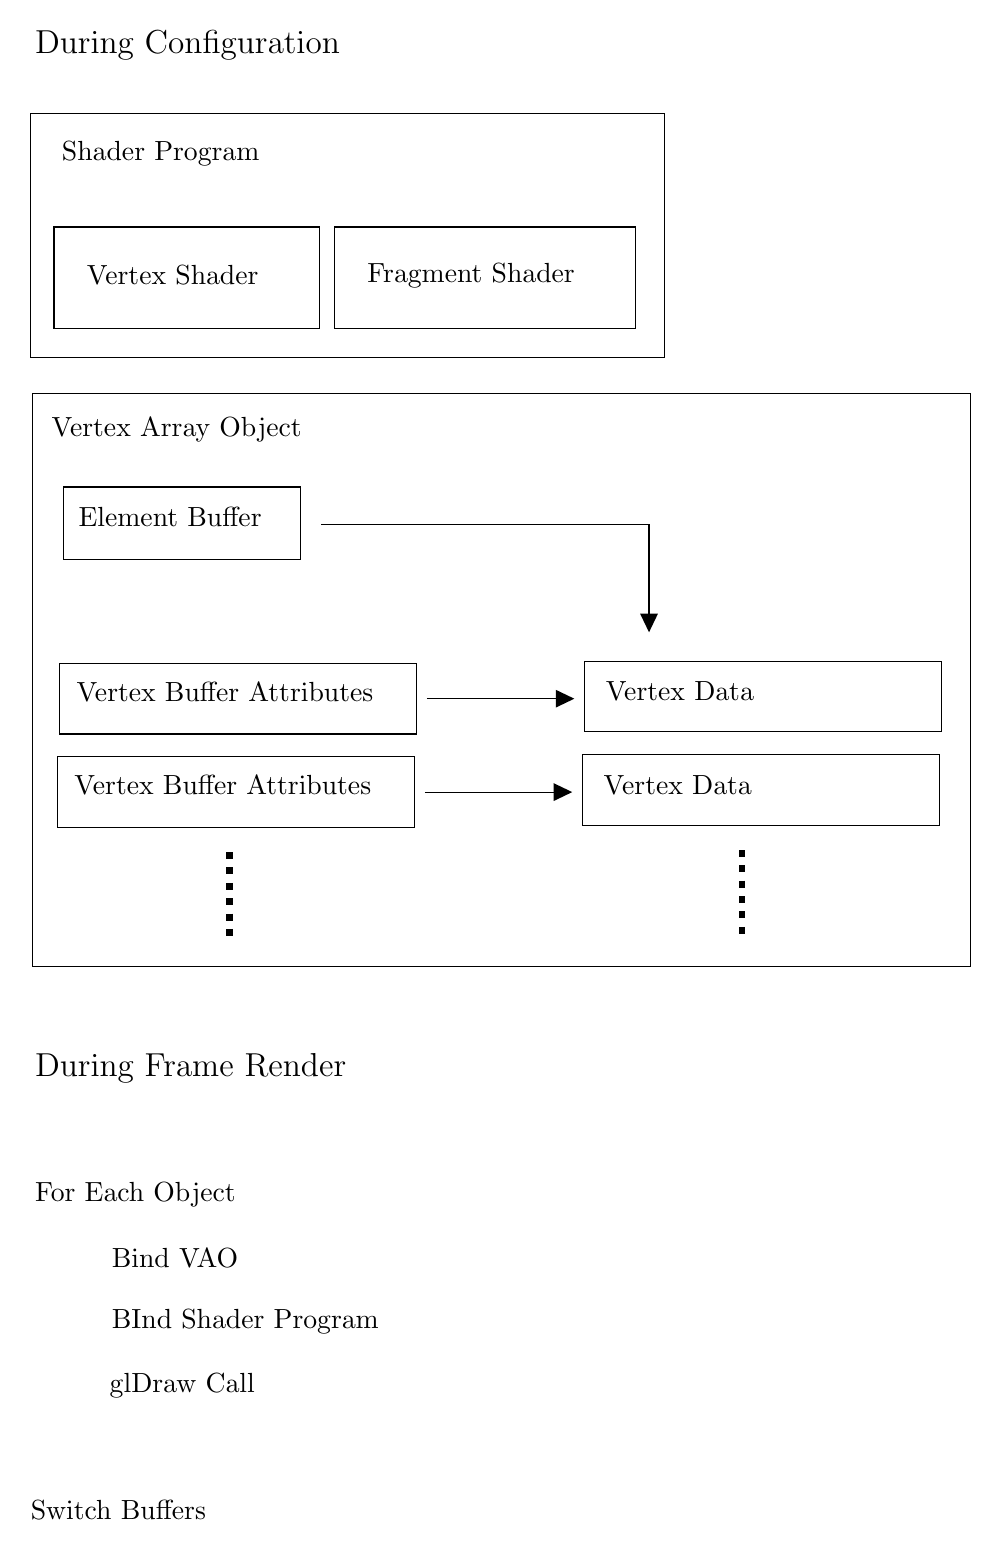
\begin{tikzpicture}[x=0.75pt,y=0.75pt,yscale=-1,xscale=1]
	%uncomment if require: \path (0,855); %set diagram left start at 0, and has height of 855
	
	%Shape: Rectangle [id:dp8822718697454482] 
	\draw   (94,64) -- (399.43,64) -- (399.43,181.77) -- (94,181.77) -- cycle ;
	%Shape: Rectangle [id:dp1908283304426488] 
	\draw   (105.43,118.77) -- (233.43,118.77) -- (233.43,167.77) -- (105.43,167.77) -- cycle ;
	
	%Shape: Rectangle [id:dp7244524197121301] 
	\draw   (240.43,118.77) -- (385.43,118.77) -- (385.43,167.77) -- (240.43,167.77) -- cycle ;
	
	%Shape: Rectangle [id:dp18755462550412272] 
	\draw   (95,199) -- (547.1,199) -- (547.1,475.03) -- (95,475.03) -- cycle ;
	%Shape: Rectangle [id:dp243965398016589] 
	\draw   (108,329) -- (280.1,329) -- (280.1,363.03) -- (108,363.03) -- cycle ;
	%Shape: Rectangle [id:dp6508857955705271] 
	\draw   (361,328) -- (533.1,328) -- (533.1,362.03) -- (361,362.03) -- cycle ;
	%Straight Lines [id:da5134438752708028] 
	\draw    (285.1,346.03) -- (353.1,346.03) ;
	\draw [shift={(356.1,346.03)}, rotate = 180] [fill={rgb, 255:red, 0; green, 0; blue, 0 }  ][line width=0.08]  [draw opacity=0] (8.93,-4.29) -- (0,0) -- (8.93,4.29) -- cycle    ;
	%Shape: Rectangle [id:dp19188267543228255] 
	\draw   (107,374) -- (279.1,374) -- (279.1,408.03) -- (107,408.03) -- cycle ;
	%Shape: Rectangle [id:dp3821137011287612] 
	\draw   (360,373) -- (532.1,373) -- (532.1,407.03) -- (360,407.03) -- cycle ;
	%Straight Lines [id:da7227305673378032] 
	\draw    (284.1,391.03) -- (352.1,391.03) ;
	\draw [shift={(355.1,391.03)}, rotate = 180] [fill={rgb, 255:red, 0; green, 0; blue, 0 }  ][line width=0.08]  [draw opacity=0] (8.93,-4.29) -- (0,0) -- (8.93,4.29) -- cycle    ;
	%Straight Lines [id:da408332221417708] 
	\draw [line width=2.25]  [dash pattern={on 2.53pt off 3.02pt}]  (190,419.93) -- (190,460.23) ;
	%Straight Lines [id:da06161874260645883] 
	\draw [line width=2.25]  [dash pattern={on 2.53pt off 3.02pt}]  (437,418.93) -- (437,459.23) ;
	%Shape: Rectangle [id:dp537977359727581] 
	\draw   (110.1,244.03) -- (224.1,244.03) -- (224.1,279.03) -- (110.1,279.03) -- cycle ;
	%Straight Lines [id:da7297870666377134] 
	\draw    (234.1,262.03) -- (392.1,262.03) ;
	%Straight Lines [id:da18316949817072714] 
	\draw    (392.1,262.03) -- (392.1,311.03) ;
	\draw [shift={(392.1,314.03)}, rotate = 270] [fill={rgb, 255:red, 0; green, 0; blue, 0 }  ][line width=0.08]  [draw opacity=0] (8.93,-4.29) -- (0,0) -- (8.93,4.29) -- cycle    ;
	
	% Text Node
	\draw (255.17,135) node [anchor=north west][inner sep=0.75pt]   [align=left] {Fragment Shader};
	% Text Node
	\draw (108,76) node [anchor=north west][inner sep=0.75pt]   [align=left] {Shader Program};
	% Text Node
	\draw (120,136) node [anchor=north west][inner sep=0.75pt]   [align=left] {Vertex Shader};
	% Text Node
	\draw (103,209) node [anchor=north west][inner sep=0.75pt]   [align=left] {Vertex Array Object};
	% Text Node
	\draw (115,336.73) node [anchor=north west][inner sep=0.75pt]   [align=left] {Vertex Buffer Attributes};
	% Text Node
	\draw (370,336.73) node [anchor=north west][inner sep=0.75pt]   [align=left] {Vertex Data};
	% Text Node
	\draw (114,381.73) node [anchor=north west][inner sep=0.75pt]   [align=left] {Vertex Buffer Attributes};
	% Text Node
	\draw (369,381.73) node [anchor=north west][inner sep=0.75pt]   [align=left] {Vertex Data};
	% Text Node
	\draw (116,252.73) node [anchor=north west][inner sep=0.75pt]   [align=left] {Element Buffer};
	% Text Node
	\draw (95,515.73) node [anchor=north west][inner sep=0.75pt]  [font=\large] [align=left] {During Frame Render};
	% Text Node
	\draw (95,23) node [anchor=north west][inner sep=0.75pt]  [font=\large] [align=left] {During Configuration};
	% Text Node
	\draw (132,609.73) node [anchor=north west][inner sep=0.75pt]   [align=left] {Bind VAO};
	% Text Node
	\draw (132,638.73) node [anchor=north west][inner sep=0.75pt]   [align=left] {BInd Shader Program};
	% Text Node
	\draw (95,577.73) node [anchor=north west][inner sep=0.75pt]   [align=left] {For Each Object};
	% Text Node
	\draw (131,669.73) node [anchor=north west][inner sep=0.75pt]   [align=left] {glDraw Call};
	% Text Node
	\draw (93,730.73) node [anchor=north west][inner sep=0.75pt]   [align=left] {Switch Buffers};
	
	
\end{tikzpicture}

	\caption{The OpenGL graphical pipeline}
\end{figure}



\section{Normalized device coordinates}
OpenGL will only process vertices with position within the normalized device coordinates range ($-1$ to $1$ on all three axis). This implies that the vertex position output from the vertex shader must be within the NDC range.

The vertex shader outputs in the NDC space, with OpenGL then transforming the vertices under NDC to screen-space coordinates using a viewport transform. The screen space vertices are rasterized and converted to fragments as inputs to the fragment shader.

\section{Buffer Objects}
There are several types of OpenGL buffer objects, each with a different buffer type. OpenGL allows one to bind multiple buffer object as long as their types are different.

Vertex array buffers represent vertex data stored on the GPU memory accessed by the vertex shader. They are stored and managed using a vertex buffer object (VBO).

Vertex array objects stores information to quickly restore a previously bounded VBO and its vertex attributes. The VAO stores all VBO vertex data binding calls and their corresponding vertex attribute calls.

Element array buffers represents index data stored on the GPU memory accessed by the OpenGL renderer. They are managed by an element buffer object (EBO). During renders, the call to \verb|glDrawElements| will draw the vertices specified by indices on the currently bound EBO and VBO. Remember that the EBO indices represents vertex indices, with each vertex possibly contains more than one vertex attribute.

\section{Shaders}
There are two ways to pass data from the application (on the CPU) to shaders (on the GPU): vertex attributes and uniforms.

Vertex attributes are buffer indices passed as inputs to the vertex shader. The buffer is taken from the currrently bound VBO with format specified by the vertex attribute pointer. Each vertex shader call will be passed a different slice of the buffer.

Uniform variables represents global data in a shader program. They are unique within a shader program, and are accessible from every shader in the shader program. Uniforms will also keep their values set by the process until explicitly changed again.

Fragment interpolation is a method used in the rasterization stage where the fragment shader inputs are interpolated against all vertex shader outputs within a primitive. This applies to every fragment shader inputs.

In general, the variable inputs to the vertex buffer is called the vertex attribute. This is often limited to 16 attributes each with a different layout metadata. When faced with a vertex buffer containing multiple interlaced vertex attributes, multiple vertex attribute pointers must be specified to detail the format of the VBO.

The vertex shader works with vertices, and each vertex often contains: a vec3 position, a vec3 color, and a vec2 texture coordinate. This implies three distinct vertex attributes for the vertex shader.

To pass additional outputs from the vertex shader to the fragment shader (albeit fragment interpolated), declare an out parameter in the vertex shader with the same name and type as an in parameter in the fragment shader.

\section{Textures}
Textures are 2D image data used to add details to model without using extra vertices.

Both textures and images can be used to store a large collection of arbitrary data used/written by shaders on the GPU. This is particularly useful in sending and receiving data from the compute shader --- for compute shaders have no inputs or outputs.

To map the vertices to the texture, we specify a texture coordinate as an additional vertex attribute to associate vertices with texture coordinates. Fragment interpolation can interpolate the texture coordinates of the remaining, non-vertex fragments.

The texture coordinate system has $(0, 0)$ on the bottom left and $(1, 1)$ on the top right.

The act of mapping from texture coordinates to texture colors is called texture sampling. There are two cases for texture sampling: texture wrapping and texture filtering.

Texture wrapping is a method to sample textures if the texture coordinates are outside of the standard texture coordinate system. The four ways OpenGL can handle such cases are to
\begin{itemize}
	\item Repeat the texture uniformly without transformations (ie, discarding the integer part of the coordinate)
	\item Repeat the texture uniformly, mirroring upon every edge. This ensures no visible crease between the repetitions.
	\item Clamping the texture coordinates to the edge of the coordinate system. This has the effect of stretching the edges of the texture.
	\item Masking the texture coordinates outside of the standard system to an uniform, user specified border color.
\end{itemize}
Each of the above option can be applied independently per coordinate axis ($(s, t)$ for a standard 2D texture).

Texture filtering is the process of mapping texture coordinates (which are floats regardless of the texture size) to texels (color data on the texture image). The options for texture filtering OpenGL provides are:
\begin{itemize}
	\item \verb|GL_NEAREST|, the default option. This results in a 8 bit, aliased look to the textures.
	\item \verb|GL_LINEAR|. This results in a blurry, interpolated but realistic look to the textures.
\end{itemize}
The texture filtering method is separately defined for magnifying and minifying textures. It is often wise to use nearest neighbor filtering when scaling down and bilinear filtering when scaling up.

Mipmaps are different resolution textures stored in a single texture file. It solves the problems with using high resolution textures for a far away object where the fragment count massively undercuts the texel counts: artifacts between fragment colors for OpenGL fails to sample between all the texels covered by the fragment, and the additional wasted memory bandwidth used in uploading a full resolution texture.

OpenGL can automatically generate mipmaps from existing textures and switch between mipmaps given the distance to the object (the mipmap is chosen to minimize the size difference between fragments and texels). Texture filtering between mipmaps is also available with the same nearest/bilinear options as regular texture filtering. Use the mipmap filtering options only on the minifying operation --- the magnifying operation doesn't use mipmaps and OpenGL will throw an error if you attempt.

To draw textures using the fragment shader, we rely on the connection between the texture objects, texture units, and samplers. Texture objects references texture memory on the GPU. They are often allocated before the render loop. Samplers are references to texture objects on the fragment shader often passed as in values. They can be used in conjunction with the \verb|texture| glsl method to sample a texture using texture coordinates. Texture units serve as connections between samplers and texture objects:
\begin{itemize}
	\item Every frame, every texture object is placed into their texture units (there are 16 available texture units)
	\item A uniform value is set on the fragment shader sampler in value that matches the index of the corresponding texture unit.
	\item OpenGL passes the texture object as a sampler in value by the linking between the texture object and texture unit (through OpenGL calls), and between the texture unit and the sampler in values (through uniform settings).
\end{itemize}

By default on most graphic drivers, the texture unit 0 is activated with the default uniform value of a sampler in value being 0, matching that of texture unit 0.

Careful around reading/loading textures with width and height not a power of 2. OpenGL defaults to aligning the pixel row start address to a power of four and thus interprets 1 byte aligned (continuous) image data incorrectly. To set one byte alignment (or to just use power of 2 texture data), call
\begin{lstlisting}[language=c++]
	glPixelStorei(GL_UNPACK_ALIGNMENT, 1);
\end{lstlisting}
before the call to load the texture image data.

\section{Transformation}
We often use 4 dimensional vectors and 4x4 matrices in OpenGL. The fourth positional component $w$ is used for depth.

% Homogeneous components
The $w$ component of a 4D vector is called the homogeneous coordinate, with vectors containing a non-zero homogeneous coordinate denoted as homogeneous vectors. These vectors have the benefits of translation under a translation matrix and the ability to be perspectively transformed to create 3D perspective projections. A vector with the homogeneous coordinate zeroed is called a direction vector for the vector can't be translated.

To extract the 3D position vector from a homogeneous vector, we divide each $(x, y, z)$ component of the homogeneous vector by its $w$ component.


The useful 4D linear transformations are
\begin{itemize}
	\item Identity, $I_4$
	\item Scaling. Non-uniform scaling has each of the axis individually scaled, while uniform scaling preserves direction and scales the axis uniformally. The scaling matrix is diagonal with the diagonal elements the scaling factors, except a scaling of 1 on the w axis.
	\item Translation. A 4x4 translation matrix with translation vector $(x, y, z)$ is
	\[
	\begin{bmatrix}
		1 & 0 & 0 & x \\
		0 & 1 & 0 & y \\
		0 & 0 & 1 & z \\
		0 & 0 & 0 & 1
	\end{bmatrix}
	\]
	Such translation matrix can only functions on homogeneous vectors.
	\item Rotation. Any 3D space rotation can be represented as a rotation of angle $\theta$ around a unit direction $d$. There exists an explicit matrix that represents such rotation --- but a quaternion solution will generally produce better results.
\end{itemize}

When combining matrix transformations, apply them in orders of: scaling, rotating, and translating to minimize undesired effects between the transformations.

In GLM, the order of the transformation function calls should be deduced in reading the matrix multiplications left to right (ie, translating, rotating, then scaling). This is because GLM applies the matrix multiplications on the right.

The matrix storage in OpenGL is column ordered, meaning that only the columns are stored as continuous data. GLM automatically exports column major data; row major data sources must be transposed before loading into OpenGL.

We can send matrix data on the CPU to the vertex shader using uniforms. On the vertex shader, we can apply the transformation to every vertex of the model by multiplying the vertex position against the transformation matrix for all vertices.

The GLM rotate function rotates counterclockwise facing (against the direction) of the specified unit direction vector. The coordinate space used by GLM is the standard OpenGL coordinates --- $x$ to the right, $y$ upwards, and $+z$ facing the front. A rotation within the $xy$ plane counterclockwise therefore uses the direction vector $(0, 0, 1)$.

\section{Coordinate System}
We usually specify coordinates in a real coordinate space, then to transform those vertex coordinates into NDC using matrix transformations. The transformations are composed of several coordinate transformation matrices, with the coordinate spaces being
\begin{itemize}
	\item Local space, with origin at the origin of the model
	\item World space, with origin at the world origin
	\item View space, with origin and direction from the camera
	\item Clip space, with perspective from the camera
	\item Screen space, with coordinates as viewport coordinates
\end{itemize}

The high-level process following a vertex coordinate in local space ending at screen space is
\begin{enumerate}
	\item The model matrix transforms the space from local to world. The matrix is determined by the location of the object's origin in world coordinates.
	\item The view matrix transforms the world space to the view space, with the matrix determined by the world location and rotation of the camera. The coordinates in view space are positioned relative to the camera's point of view.
	\item The projection matrix transforms the view space into the clip space (also known as the NDC). The matrix used can add perspective to the coordinates. Clipping is done on the outputs of the projection matrix.
\end{enumerate}

\paragraph{Projection Matrix}
The output of the vertex shader (determined lastly by the projection matrix on the view space) undergoes clipping that retains only the vertices within the NDC. A primitive that is partially clipped will be automatically reconstructed by OpenGL into other triangles that fits in the clipping space.

The viewing box --- area where the projection matrix maps into the unclipped NDC --- is called the frustum of the projection matrix.

Orthographic projection has a rectangular, uniform frustum. It orthogonally projects/maps vertices within its frustum onto the clip space plane with no modifications to the w component. The projection matrix is uniquely defined by the near and far plane's width, height, and their respective distances.

Perspective projection introduces perspective into the transformation. It has a non-uniform, cone like frustum that shrinks further objects more than nearer objects through increasing their mapped $w$ values. The result is that at every depth $w$, the clip space ranges from $-w$ to $w$ instead of a uniform clip space range at every depth. The perspective projection matrix is uniquely defined by the FOV angle, aspect ratio of the near plane, and the distances of the near and far planes.

For a perspective projection, the FOV determines the relative angle width of the cone shaped frustum: a higher FOV increases the visible plane at every distance, hence decreasing the size of objects; a lower FOV decreases the visible plane at every distance, hence increasing the size of objects. The perspective matrix's aspect ratio determines the relative aspect ratio of the near and far planes. With the viewport size unchanged: increasing the aspect ratio increases the visible area but squishes along the horizontal direction for the wider visible area is now mapped to the same number of horizontal pixels; decreasing the aspect ratio decreases the visible area and stretches along the horizontal direction for the narrower visible area is mapped to the horizontal pixels.

\paragraph{Handness}
OpenGL uses a right-handed system. With the positive x to the right, positive y upwards, and positive z axis out of the screen towards you. Alternatively, a left-handed system has the positive z axis pointing into the screen. Both Direct3D and the NDC of OpenGL uses the left-handed system --- the projection matrix of GLM switches the handedness from right to left.

\paragraph{Depth Buffer}
For OpenGL does not guarantee the order at which primitives (and even fragments in a single primitive) are drawn, we must use a depth buffer (or z buffer) to solve the problem of rendering overlapping polygons.

The depth buffer is analogous to the color buffer, with a buffer size the same as the amount of pixels in the viewport. The depth of a fragment (representing a potential pixel) is its $z$ viewport coordinate (normalized from $-1$ to $1$, of course) --- this is why the depth buffer is common known as the z buffer.

When OpenGl's optional depth testing feature is turned on, the step to render the fragment shader output changes to
\begin{enumerate}
	\item The depth (z value) and screen position of the fragment is calculated
	\item The depth is compared with the existing depth value in the depth buffer
	\item If the depth value is lower (closer to the screen) then the one in the depth buffer, this new fragment depth will overwrite the depth in the buffer and the fragment color is drawn to the color buffer
	\item Otherwise, the fragment color and depth information is discarded.
\end{enumerate}

The depth buffer testing feature is by default, off. Also remember to clear the depth buffer between render frames.

\section{Camera}
For the view matrix transforms from the world space to the camera POV view space, we wish to generate the view matrix from the positions and rotations of the camera.

To create the view matrix, we need a coordinate system from the camera's point of view. To do this we need the following information: the camera position in world space, a direction vector (which is the negated target direction vector), a right vector, and an up vector.

Here is the procedure to compute the above camera coordinate space:
\begin{enumerate}
	\item The camera position is just its world space position --- a vector from the world origin to the camera position
	\item The camera direction is computed by subtracting the target position from the camera position and normalizing. This results in a direction vector from the target to the camera, which is a vector opposite to the camera facing direction and serves as the positive z axis (the negation is due to the OpenGL coordinate system by default, having the camera point towards negative z).
	\item To get a right vector, we cross product the world space up vector with the camera direction vector and normalizing. This right vector serves as the x axis in the camera's coordinate system.
	\item To get an up vector, we cross the direction vector with the right vector. This serves as the y axis in the camera's coordinate system.
\end{enumerate}

We can then create a lookat matrix that serves to be our view matrix. The lookat matrix inverts the camera position, changes the basis to the camera's coordinate basis. Using the four helper camera vectors: position $P$, direction $D$, right $R$, and up $U$, we can create this view matrix by
\[
	V = \begin{bmatrix}
		R_x & R_y & R_z & 0\\
		U_x & U_y & U_z & 0\\
		D_x & D_y & D_z & 0\\
		0 & 0 & 0 & 1
	\end{bmatrix} \times \begin{bmatrix}
		1 & 0 & 0 & -P_x\\
		0 & 1 & 0 & -P_y\\
		0 & 0 & 1 & -P_z\\
		0 & 0 & 0 & 1
	\end{bmatrix}
\]

Notice that the right matrix is the inverted camera translation matrix. The left matrix is a change fo basis matrix that is transposed (the reason for the transpose is to invert the matrix, which because it is orthogonal, will be equivalent to an inverse).

For a realistic FPS control scheme, we set the target position to be the sum of the camera position and a unit direction vector. To compute and control this direction vector using the yaw $\theta$ and pitch $\phi$ angles (inputs from the mouse), we can use the formula
\[
	D = \begin{bmatrix}
		\cos \phi \cos \theta\\
		\sin \phi\\
		\cos \phi \sin \theta
	\end{bmatrix}
\]
where the theta is the counterclockwise angle from the x axis, and the pitch is the signed angle from the xz plane.

In updating the yaw and pitch values, the pitch must be clamped to not reach exactly $\pm 90$ degrees for the lookAt function will not function when the direction vector equals the up vector.

Notice for GLFW. We will need to filter out the first mouse movement callback invocation, for the new position values will not be close to the initial values will thus create a large jitter in the camera upon window focus.

The limitations of this camera system include:
\begin{itemize}
	\item Inability to look directly up or down.
	\item Cannot incorporate roll with a static up vector.
	\item Numeric instabilities when pitch is close to the constraint, and unclamped yaw may be problematic when the value becomes extremely large.
\end{itemize}

\section{Review}









\end{document}